\documentclass[a4paper,12pt]{article}
\usepackage[utf8]{inputenc}
\usepackage{amssymb,amsmath,uniinput,graphicx}
\usepackage[section]{placeins}
\usepackage[ngerman]{babel}
% for uniinput: https://wiki.neo-layout.org/browser/latex/Standard-LaTeX
\usepackage{hyperref}
%\usepackage{multirow}
\usepackage{units}
\usepackage[left=3cm,right=3cm,top=3cm,bottom=3cm]{geometry}
\renewcommand{\familydefault}{\sfdefault}
\setlength{\belowcaptionskip}{6pt}
\hypersetup{pdfinfo = {
	Title={Versuchsprotokoll zur Paulschen Teilchenfalle},
	Author={Knut Kiesel, Tobias Pook},
	Keywords={Teilchenfalle}
}}

\title{Laborpraktikum Teilchenphysik\\ Paulsche Teilchenfalle}
\author{Knut Kiesel\\Tobias Pook}
\date{\today}

\begin{document}
\maketitle
\thispagestyle{empty}
\newpage
\tableofcontents
\setcounter{page}{1}
\newpage 

\section{Ziel der Messung} % max 1 Seite
Ziel des Versuches ist die Speicherung von elektrisch geladenen Teilchen und die Bestimmung des Ladungs-Massen Verhältnisses.
Um die Teilchen in einem räumlich begrenzten Feld zu halten, ist ein statisches elektrisches Feld nicht ausreichend, da man damit keine Potentialminima schaffen kann.
Eine Möglichkeit dennoch Teilchen zu fangen ist das Anlegen von phasenverschobenen Wechselspannungen und Gleichspannungen, wobei bei richtiger Einstellungen der Spannungen und Frequenzen die Teilchen stabil in der Falle bleiben.
Konkret wurden beim durchgeführten Experiment der meta-stabile Bereich eines rotierenden Sattelpotential genutzt um Teilchen zu speichern.
Für jede räumliche Komponente $i\in\{x,y,z\}$ lautet die Bewegungsgleichung
\begin{align*}\label{mastergleichung}
	\frac{4}{mΩ^2} |\vec{F}_i| + \left( a_i -2q_i \cos\left( 2\xi_i \right) \right) i  + 2k_L \frac{dx}{d\xi_i} + \frac{d^2x}{d\xi_i^2} = B\cos\left( \frac{2ω_W}{Ω}ξ_i \right)
\end{align*}
mit dem gleichstromabhängigen Koeffizienten $a_i = \frac{16KqU_{G,i}}{3Ω^2mr_0^2}$,
dem wechselstromabhängigen Koeffizienten  $q_i = -\frac{4kqU_i}{Ω^2mr_0^2}$,
dem Antribskoeffienzenten $B = \frac{2qU_W}{r_0mΩ^2}$,
dem Luftreibungskoeffizient $k_L = \frac{6πηR}{mΩ}$, der Winkelfrequenz der Dreiphasenspannung $Ω$,
der Winkelfrequenz der zusätzlich an einem Plattenpaar angelegten Wechselspannung $ω_W$
und der normalisierten Zeit $ξ = \frac{Ωt}{2}$.
Die Kraft $\vec{F}$ ist die Gewichtskraft (die nur auf die z-Komponente Auswirkungen hat).
Die Grundschwingung der Lösung wird durch $β_i = \sqrt{a_i + \frac{q_i^2}{2}}$ beschrieben.
Durch Anlegen geeigneter Frequenzen und Spannungen und das Beobachten der Entstehenden Teilchenbewegungen kann mit unterschiedlichen Methoden das Verhältnis von Ladung zur Masse bestimmt werden.


\section{Aufbau und Durchführung}
Die z-Achse verläuft vertikal, die y-Achse ist die Blickrichtung, und die x-Achse liegt senkrecht zu den beiden übrigen.

Die Falle wird aus sechs Kupferringen und 12 Verbindungsstücken zu einem Würfel geklebt.
Nach dem Anlöten und Isolieren der Anschlusskabel wird die Falle mit schwarzem Lack angemalt, um Steulicht in der Kammer zu verringern.
Die Falle wird mittig über der Öffnung für die Spritze an den Anschlusskabeln befestigt, und die Plattform von unten an die Spannungsversorgung angeschlossen (siehe Bild \ref{fallenbild}), welche je nach Hebelstellung die Gleichspannungen oder die zusätzliche Wechselspannung zur Dreiphasenspannung hinzufügt.
Die Dreiphasenspannung, im folgenden auch Fokussierspannung genannt, besteht aus drei Wechselpannungsquellen die mit einem konstanten Phasenunterschied von $120°$ betrieben werden. Die Amplitude kann dabei für jedes Flächenpaar individuell eingestellt werden. 

\begin{figure}[htb]
		\centering
		\includegraphics[width=0.3\textwidth]{falle.jpg}
		\caption{Versuchsaufbau der Paulschen Teilchenfalle}
		\label{fallenbild}
\end{figure}

Im Spannungsgenerator gibt es mehrere Möglichkeiten die Gleichspannung anzulegen:
Man kann sie auf den beiden gegenüber liegenden Seiten oder zwischen zwei gegenüberliegenden Seiten anbringen.
Die Verschaltung kann man Bild \ref{verschaltung} entnehmen.
\begin{figure}[htb]
		\centering
		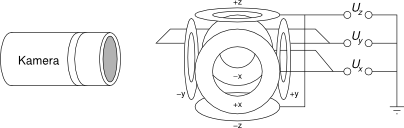
\includegraphics{Schaltbild_3Phasen.png}
		\caption{Verschaltung im Generator}
		\label{verschaltung}
\end{figure}

Aus Sicherheitsgründen wird die Falle durch eine durchsichtige Acrylhaube abgedeckt. Die Haube wurde zusätzlich mit schwarzem Klebeband verkleidet, mit zwei Öffnungen eine für die seitliche Beobachtung der Falle und eine für die von oben angebrachte Lampe.  
Der Versuch wird mit Aluminum Pulver durchgeführt, dieses wird mittels einer Spritze durch eine Öffnung unterhalb der Falle eingebracht. Da zwischen Öffnung und dem stabilen Bereich der Teilchenfalle ein Abstand von ca. $\unit(2.5){cm}$  besteht wurden die Teilchen durch anschnippsen der Spritze in die Falle geschleudert.




\section{Ergebnisse}
Mit einem Messschieber wird der Plattenabstand der Teilchenfalle auf $\unit[(3.05±0.02)]{cm}$ abgeschätzt.
\subsection{Bahnbeschreibung}
Ellipsen
In den meisten Fällen beschreiben die einefangenen Teilchen eine elliptische Teilchenbahn, dabei lässt sich der Radius und die Exzentrizität durch das Verhältnis der angelegten Potenziale in der Fokusierspannung


Lissajous Figuren
Lissajous Figuren entstehen bei der Überlagerung harmonischer Schwingungen wenn das Verhältnis der Frequenzen rational ist, sich also durch einen ganzzahligen Bruch darstellen lässt. 
In diesem Fall bildet die Teilchenbahn eine geschlossene
Figur. Die möglichen Formen der Figuren sind sehr vielfältig und hängen vom Frequenzverhältnis und dem Phasenunterschied der Schwingungen ab. 

\begin{figure}[htb]
		\centering
		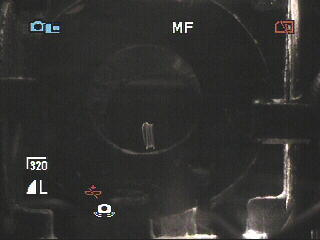
\includegraphics{lisa1.jpg}
		\caption{Beispiel für das auftreten einer Lissajous Figur}
		\label{Lissjous}
\end{figure}
, Kristallstrukturen, Elipsen: Spannungen nicht gleich\dots
\subsection{Kompensation der Gewichtskraft}
In Gleichung (\ref{mastergleichung}) wird der Einfluss der Luftreibung vernachlässigt und ein Näherungsansatz der Form $z(ξ_z) = Z(ξ_z)+d(ξ_z)$ durchgeführt.
Die z-Komponente wird nun durch 
\begin{align*}
	Z(ξ) = Z_0\sin(β_zξ) - \frac{4|\vec{F_z}|}{mβ_zΩ^2}
\end{align*}
beschrieben.
Man sieht, dass die Schwingung um einen konstanten Term verschoben ist, der von $a_z$ und $q_z$ abhängt.
Diese Abhängigkeit besteht nicht mehr, wenn gilt:
\begin{align*}\label{kraftgleichgew}
	|\vec{F}_{z}| = |\vec{F_G} + \vec{F_{qE}}| = 0
\end{align*}

% vorzeichen?
\begin{figure}[htb]
		\centering
		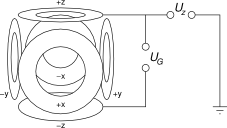
\includegraphics{Schaltbild_Z_Kompensation.png}
		\caption{Schaltbild Z-Kompensation}
		\label{schalt-z}
\end{figure}
Die Fokussierspannung wird bei $\unit[(1000±50)]{V}$ für alle Flächenpaare betrieben.
Zu der Fokussierspannung wird nun ein zusätzlicher Potentialunterschied zwischen den beiden z-Komponenten angeschlossen 
(siehe \ref{schalt-z}), dieser wird solange erhöht bis die Gravitationskraft 
kompensiert wird. Dies kann dadurch überprüft werden, dass sich der Mittelpunkt der Teilchenschwingung bei Änderung 
der Amplitude der Z-Komponente der 3-Phasenspannung nicht mehr ändert.
Die Gleichspannung hat während des Versuchs teilweise 
stark geschwankt. Die effektive Spannung wurde durch notieren der angezeigten Werte in einem Zeitraum 
von ca. $\unit[20]{s}$ und anschliessendem Mitteln bestimmt. Da die Teilchen oft wegen spontaner Spannugsschwankungen 
der Quelle verloren gegangen sind konnte der Bereich, in dem die Gravitationskraft kompensiert wird, nicht in feineren Spannungsabschnitten untersucht werden.
Da so nicht abzuschätzen ist wie exakt der Wert für die Kompensationsspannung $U_G$ getroffen wurde, wird als Fehler die mittlere Differenz zu den nächstliegenden 
$UG$ gewählt, bei dem wieder Bewegungen des Schwingungsmittelpunkt bei variation  der Fokussierspannung $U_z$ zu beobachten sind.
Die Messung wurde für mehrere gleichzeitig gefangene Teilchen durchgeführt und die Spannung erhöht bis alle Teilchen den Stabilitätsbereich verlassen haben.
Wegen den bereits erwähnten Schwankungen konnte die Messung nur für 2 Teilchen erfolgreich durchgeführt werden.
	
	\begin{table}
	\centering
	\begin{tabular}{ l | c | r }
		$U_{G} [V]$ & $\sigma_{U_{G}}[V]$ & Verhalten des Bahnmittelpunkt bei änderung von U_z  \\
		\hline
		45 & 5 & Teilchen 1,2 Bewegung   \\
		92 & 8 & Teilchen 1 still,Teilchen 2 Bewegung \\
		168 & 4 & Teilchen 1,2 Bewegung    \\
		228 & 3 & Teilchen 1,2 Bewegung \\
		273 & 5 & Teilchen 1 verloren , Teilchen 2 still \\
	\end{tabular}
\caption{Messpunkte der Z-Kompensationsmessung}
\label{tab:z-komp-measure}
\end{table}
Aus \ref{kraftgleichgew} lässt sich direkt eine Formel für die spezifische Ladung des untersuchten Teilchen herleiten:
\begin{align*}\label{zspezm}
	\frac{q}{m} = \frac{g\cdotcd  d}{U_{G}}
\end{align*}
Beim berechnen der Ergebnisse wurde die Erdbeschleunigung mit $9.81$ als fehlerfrei angenommen, der Plattenabstand wurde zu $\unit[(3.05±0.02)]{cm}$ abgeschätzt. 
Die erechneten Werte können \ref{z-komp-result} entnommen werden.

	\begin{table}
	\centering
	\begin{tabular}{ l | c | c| r }
		$U_{G,komp} [V]$ & $\sigma_{U_{G,komp}}[V]$ & $\frac{q}{m}[\frac{C}{kg}]$ & $\frac{\sigma_{\frac{q}{m}}}{\frac{q}{m}}$  \\
		\hline
		\hline
		Teilchen 1 \\
		92 & 61.5 & 0.0 & 0.0 \\
		\hline
		Teilchen 2 \\
		273 & 45 & 0.0 & 0.0 \\
	\end{tabular}
\caption{Messpunkte der Z-Kompensationsmessung}
\label{tab:z-komp-result}
\end{table}




\subsection{Resonanz}
In diesem Versuchsteil wurde zusätzlich zur Fokusierspannung  eine Wechselspannung zwischen dem Flächenpaar entlang der X-Achse angelegt. Damit vereinfacht sich \ref{mastergleichung} zu: 
\begin{align*}\label{resgleichung}
	\left( a_i -2q_i \cos\left( 2\xi_i \right) \right) i  + 2k_L \frac{dx}{d\xi_i} + \frac{d^2x}{d\xi_i^2} = B\cos\left( \frac{2ω_W}{Ω}ξ_i \right)
\end{align*}
Die Teilchenbahn wird also durch eine erzwungene Schwingung moduliert, die Lösung von \ref{resgleichung} ist gegben durch:
\begin{align*}\label{resgleichung}
	X(\xi_x) = X_0( \beta_x,\omega_W ) \cdot B \cdot cos(2\frac{\omega_W}{\Omega}\xi_x - \Phi(\beta_x,\omega_W))
	\\
	 tan\Phi(\beta_x,\omega_W) = \frac{4 k_L \Omega \omega_W}{\beta_x^{2}\Omega_x^{2}} 
	 \\
	  X_0 = \frac{1}{\sqrt{16\omega^{4}_W\Omega^{-4}+\beta^{4}_x+16\Omega^{-2}k_L\omega^{2}_W-8\Omega^{-2}\beta^{2}_x\omega^{2}_W}}
\end{align*}
bei einer Frequenz von $\omega^{res}_W = \frac{\Omega}{2}\sqrt{\beta^{2}_x-2k^{2}_L} $ tritt eine resonante 
Verstärkung der Oszillation auf und die Teilchenbahn erreicht ihre maximale Auslenkung.
\begin{align*}\label{Amax}
	A_{max} = \frac{B}{2k_L\sqrt{\beta^{2}_x-k^{2}_L}}
\end{align*}
Zur späteren digitalen Vermessung der Auslenkung wurden mit einer Digitalkamera Fotos der Teilchenbahn angefertigt.
Dazu wurde vor durchführung des Versuchs die Falle entfernt und eine Längenskala auf Höhe der Fallenmitte senkrecht zur Kamerablickrichtung platziert.  
Da sowohl die Kameraposition als auch die Teilchenfalle nicht mehr bewegt werden, kann aus diesen Bildern ein Zusammenhang zwischen Pixeln pro cm in der Beobachtungsebene 
bestimmt werden.
\\
Aus den gemessenen Werten für $\omega^{res}_W$ und $A_{max}$ lässt sich eine weitere Formel zur bestimmmung der spezifischen Masse des Teilchen herleiten. 
Für die Vakuummessung, bzw. als Näherung für den Aufbau in Luft, kann die Luftreibung vernachlässigt werden ($k_L = 0$).  
\begin{align*}\label{resspezm}
	\frac{q}{m} = -\frac{\Omega r^{2}_0 \omega^{res}_W}{\sqrt{2} K U_x}
\end{align*}

\subsection{Stabilitätsdiagramm}

\section{Vergleich der Messungen}

\section{Fazit}
Die Versuchsdurchführung war dadurch geprägt das die Spannungsquelle nur stark schwankende Ausgangsspannungen geliefert hat. Besonders ein reglemäßiges plötliches Abfallen der Fokussierspannung für ein 
Flächenpaar hat zu regelmäßigem Verlust der Teilchen geführt. Insbesondere die Resonanzmessung und die Stabiliätsmessung waren oft nicht durchzuführen, weil ein langfristiges einfangen der Teilchen nicht
möglich war.

% max 30 seiten
\end{document}
